\documentclass{article}


\usepackage{authblk}
\usepackage{listings, chngcntr}
\usepackage{multicol}
\usepackage{textcomp}
\usepackage{float}
\usepackage[T1]{fontenc}
\usepackage{indentfirst}
\usepackage{graphicx}
\usepackage{array}
\usepackage{caption} 
\usepackage{hyperref}
\usepackage{verbatim}
\usepackage{float}
\usepackage{subcaption}
\usepackage{gensymb}
\usepackage{amsmath}
\usepackage{geometry}
\usepackage{multirow}
\usepackage{listings}


\geometry{
    a4paper,
    left=30mm,
    right=30mm,
    top=30mm,
    bottom=40mm
}

\begin{document}

\title{Noise Floor Estimation and The Performance Check of the Operational Amplifier}
\author[1]{Woojin Han}
\affil[1]{Seoul National University, Seoul 151-747, Korea}
\maketitle

\begin{abstract}
    The low noise amplifying system takes a major place in the high-resolution physics experiment.
    Operational Amplifier, which is composed of a resistance and the voltage source has inevitable errors to have a rock bottom of a noise.
    To magnify the signal-to-noise ratio larger, the unnecessary error parts should be controlled better.
    In this report, the noise floor detection is performed by changing the capacitance value of the circuit, detailly the length of a cable is varied.
    With the finely controlled noise, the lock-in detection is digitally calculated from the cross-input of the signal via Visa communication.
    Therefore, the internal resistance of the custom operational amplifier is calculated, which has the order of $100 M \Omega$.
\end{abstract}


\section{Introduction}
In signal theory, the experimental noise is considered inevitable.
There are two kinds of noises to dissert on, which can be reduced enough by experimental setup to be neglected.
The others are mainly for thermal reasons and if it contains semiconductor shot and flicker noise also takes place in inescapable noise, called noise floor.
As it is called noise floor, there are no ways to reduce that noise without making the system $0K$ or using the ideal instruments.
Since the experimental setup has its limit, hitting the noise floor is considered a great preset to experiment.
The shot and flicker noises are calculated in a semiconductor system, which converges to the thermal noise via frequency increases, dealing with thermal noise in the minimized system helps successors to greet the signal and noise theory better.
Through this report, the noise floor estimation by thermal calculation and impedance calculation is performed with order checks, and the availability of a custom operational amplifier(op-amp) has been discussed.

\section{Methods}
There are two experiments, noise floor measure by ground input detection and resistance measurement corrected by the noise is performed.
The portable oscilloscope, DHO924 from Rigol is used, and its performance is opened by the producer (\cite{Rigol}).
Below the $5mV/div$ condition, DC gain Accuracy is reported as $2\%$ which is considered at ground input experiment.
Above the $5mV/div$ condition, DC gain Accuracy is $1\%$ where the resistance measurement counts.
The op-amp is custom-made from Jeonbuk National University, and its error is reported as $i_n = 5 fA/\sqrt{\mathrm{Hz}}$, $e_n = 3 nV/\sqrt{\mathrm{Hz}}$.

\subsection{Noise Floor Detection}
Fig \ref{fig: noise floor circuit plot}. shows the schematic plot of the circuit.
$R1$ is the sample resistance, which is 100$M\Omega$ dominates the cable resistance.
$C$ is the cable capacitance, which is expected linearly dependent on the cable length and also dominates the sample capacitance.
This deduction is legitimate due to the big gap between the length of the sample and the cables.
The results are discussed below at \ref{subsection: Noise Floor Detection}.
\begin{figure}[H]
    \centering
    \begin{subfigure}[b]{7cm}
        \centering
        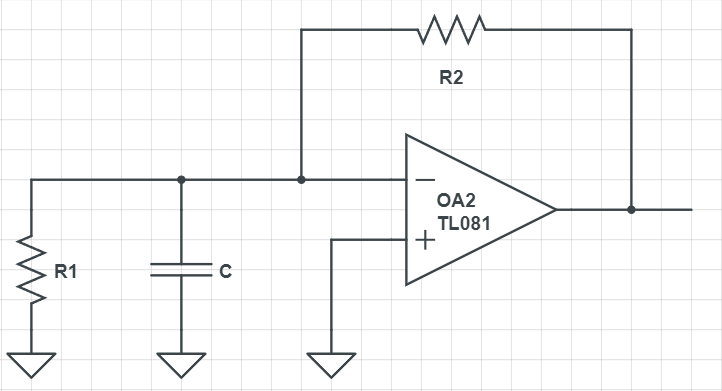
\includegraphics[width=7cm]{./figs/ciruit.png}
        \caption{}
    \end{subfigure}
    \hfill
    \caption{Schematic diagram of the circuit}
    \label{fig: noise floor circuit plot}
\end{figure}

\subsection{Resistance Measurement}
Fig \ref{fig: resistance measurement plot}. shows the schematic plot of the circuit.
$RS$ is the sample resistance, which is denoted as 100$M\Omega$.
$VS$ is the voltage source, which amplitude and frequency can be freely modified.
$V1$ and $V2$ each are measured by an oscilloscope, and the lock-in detection is calculated.
The results are discussed below at \ref{subsection: Resistance Measurement}.
\begin{figure}[H]
    \centering
    \begin{subfigure}[b]{7cm}
        \centering
        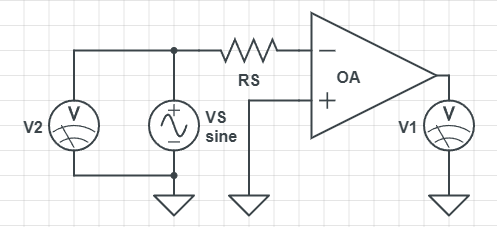
\includegraphics[width=7cm]{./figs/circuit2.png}
        \caption{}
    \end{subfigure}
    \hfill
    \caption{Schematic diagram of the circuit}
    \label{fig: resistance measurement plot}
\end{figure}

\section{Results and Discussion}
\subsection{Noise Floor Detection}
Two kinds of cable are crossly used to double-check the error mitigation via capacitance.
Long cable which have length of $L_l = 2930 \pm 5 [mm]$, and short cable with $L_s = 937 \pm 5 [mm]$.
By changing the cables while fixing the length kind of it, the ground error is measured three times each.
The cables are connected resistance to the amplifier and the amplifier to the oscilloscope.
Cable 1 denotes the cable to the amplifier from the resistance, which is affected by $e_n$.
Cable 2 is the cable from the amplifier to the oscilloscope, but its capacitance does not affect the ground noise explicitly.
Just to ensure the fact, Cable 2 also differed to be measured.
The result of each condition is written in Fig. \ref{fig: ground error result}.
The noise raw plot in the time series is shown in Fig \ref{fig: ground error scatter plot}.
Since the scatter plot itself does not contain rich enough data, the plot of a condition represents others.
The error bar is plotted, but too small to be neglected, due to the high resolution of the oscilloscope.
The noise floor has four different major dependencies.
The basic current noise $i_n$ comes first, and the thermal fluctuation of current flow from the resisters follows.
$i_{n_T} = \sqrt{\frac{4k_B T}{R_s}}$, $T$ refers to the sample temperature, where $k_B$ is Boltzmann constant.
Moreover, Amplifier voltage noise propagates to the sample and has a current noise of $i_{n_V}=\frac{e_n}{R_s}$.
Lastly, the cable affects the capacitance of the circuit and reactance to the voltage noise.
$i_{n_C} = e_n 2 \pi f C_s$

By using the propagation of uncertainty, total error can be calculated as Eq. \ref{eq: current noise}.

\begin{equation}
    {i_{n_{tot}}}^2 =  i_n^2 + \left(\sqrt{4k_B T \frac{1}{R_s}}\right)^2 + \left( \sqrt{4 k_B T \frac{1}{R_f}}\right)^2 + \left( \frac{e_n}{R_s}\right)^2 + \left( e_n 2\pi f C_s \right)^2
    \label{eq: current noise}
\end{equation}

Except for the last term, the noise is from inevitable sources such as temperature or voltage vibration.
So, if the change of the cable length affects the error dominantly the experiment set can be considered great.
As expected, the change of cable 2 is not affecting the main error, by comparing results of (1,2,3) and (7,8,9) in Fig. \ref{fig: ground error result}.
When cable 1 changes to the longer object, the error increases significantly, so that the apparatus is well set.
The cable capacitance is approximately $500 pF$, where the bandwidth frequency of $50 kHz$,
$V_{n_C} = 0.4 [mV]$. Which order fits well with the experiment result, the resistance calculation is now prepared.

\label{subsection: Noise Floor Detection}
\begin{figure}[H]
    \centering
    \begin{subfigure}[b]{14cm}
        \centering
        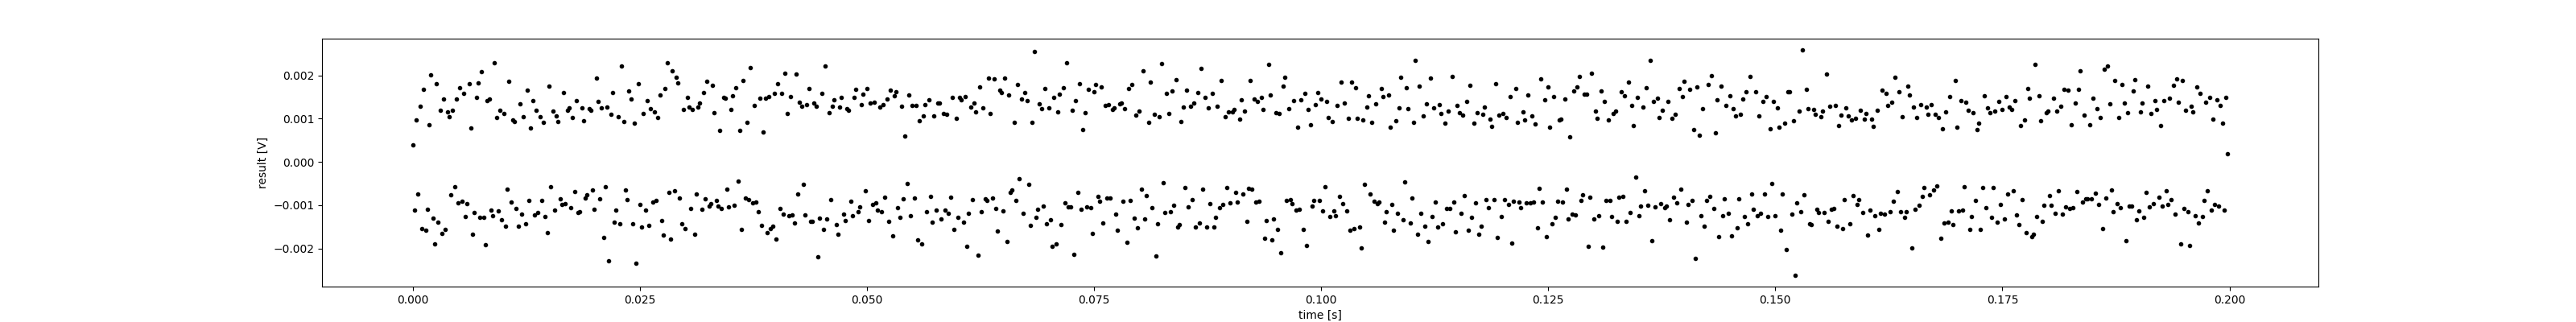
\includegraphics[width=14cm]{./figs/figure0.png}
        \caption{}
    \end{subfigure}
    \hfill
    \caption{Scatter plot of a ground error Voltage [V] - time [s]. Long cable is used, in sample resistance 100 $M \Omega$, amplifier gain of $10^6 V/A$.}
    \label{fig: ground error scatter plot}
\end{figure}

\begin{figure}[H]
    \centering
    \begin{tabular}{c|c|c|c}
        \centering
          & cable 1 & cable 2 & $\sigma_V [mV]$ \\ \hline
        1 & short   & short   & 0.7025          \\ \hline
        2 & short   & short   & 0.6960          \\ \hline
        3 & short   & short   & 0.6862          \\ \hline
        4 & long    & short   & 1.319           \\ \hline
        5 & long    & short   & 1.334           \\ \hline
        6 & long    & short   & 1.328           \\ \hline
        7 & short   & long    & 0.7258          \\ \hline
        8 & short   & long    & 0.7200          \\ \hline
        9 & short   & long    & 0.7173          \\ \hline
    \end{tabular}
    \caption{Noise floor experiment results in different cable conditions, cable 1 is the cable before the amplifier, cable 2 is cable to oscilloscope}
    \label{fig: ground error result}
\end{figure}

\subsection{Resistance Measurement}
\label{subsection: Resistance Measurement}

Lock-in detection can be performed in analog calculation circuits, which are supported by plenty of apparatus.
But, to maintain the ability to control Visa communication, the lock-in detection is performed in the digital calculation.
As in Fig. \ref{fig: resistance measurement plot}, the voltage measurement results from $V1$ and $V2$ probes are both inputted to the oscilloscope.
Then, by considering the phase shifts the Riemann integral between two signals is calculated.
Fig. \ref{fig: lock-in detection} shows the Voltage-time scatter plot of a measured object.
As the frequency scale is low enough in comparison with the sampling rate, the Riemann integral can be considered accurate enough.
Voltage amplitude controlled from 5 [mV] to 205 [mV], in arithmetic progression of 5 [mV], in 1 [kHz] to 20 [kHz] with 1 [kHz] gap, 820 times.
In each condition, 1024 points are sampled from the oscilloscope, and calculated.
In Fig. \ref{fig: resistance measurement result} (a), the lock-in voltage[V] - current[A] is plotted.
From the linear regression, the sample resistance is measured as $140\pm 1 [M \Omega]$, which has a similar order but is significantly shifted positively.
I claim that this result is from the performance interval of high input voltage and the high gain condition.
Fig. \ref{fig: resistance measurement result} (b) shows the phase shift between the input signal and the result current having a large gap from $\pi/2$, which can be considered an anomaly.
The unexpected phase shift occurs from the internal resistance of the op-amp when the sample resistance is not small enough to be neglected.
From the experimental result, I can find the custom operational amplifier is using about $10^10 \Omega$ resistance internally, and therefore the gain rate is not performing as well as the gauge says.
In the trust of a $100M \Omega$ resistance label, the gain has a loss of $30\%$ which is from the compatible resistance of an apparatus.

\begin{figure}[H]
    \centering
    \begin{subfigure}[b]{14cm}
        \centering
        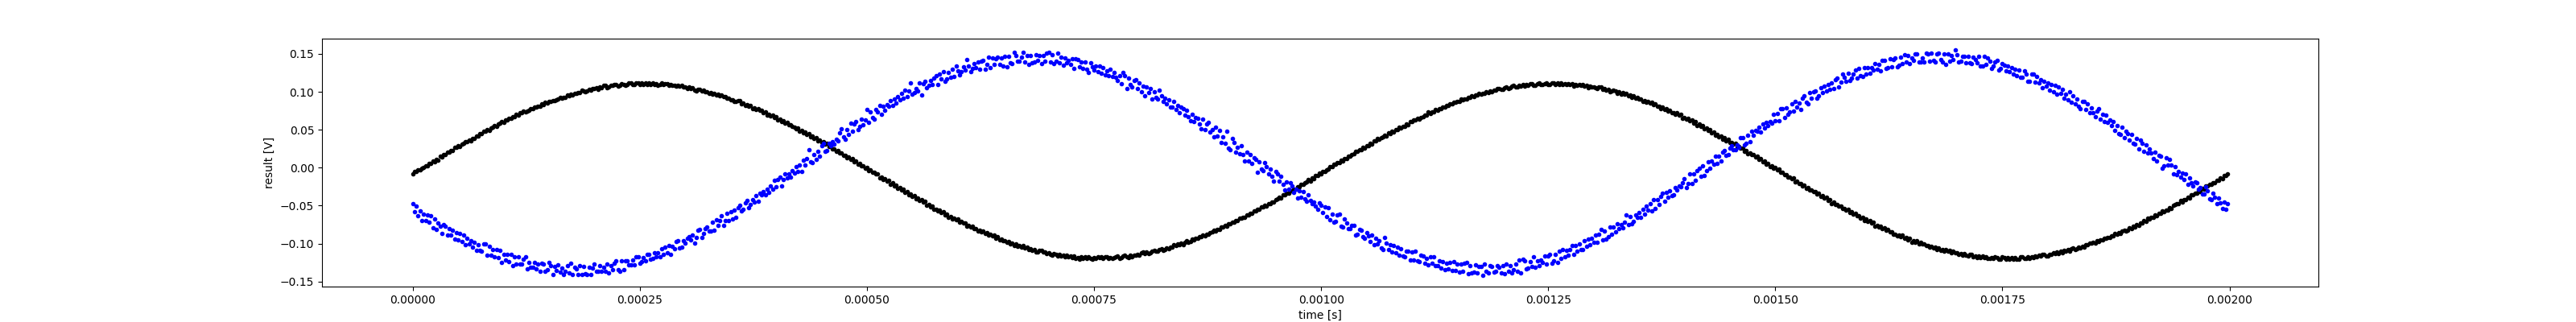
\includegraphics[width=14cm]{./figs/V-t plot sine 140 [mV] 1 [kHz].png}
        \caption{}
    \end{subfigure}
    \hfill
    \caption{
        Scatter plot of a $100M \Omega$ resistance, Voltage [V] - time [s].
        The black line refers to an input signal, and the blue line represents the output signal, amplifier gain of $10^8 V/A$.
        The input voltage is 1 [kHz], with an amplitude of 140 [mV].
    }
    \label{fig: lock-in detection}
\end{figure}
\begin{figure}[H]
    \centering
    \begin{subfigure}[b]{7cm}
        \centering
        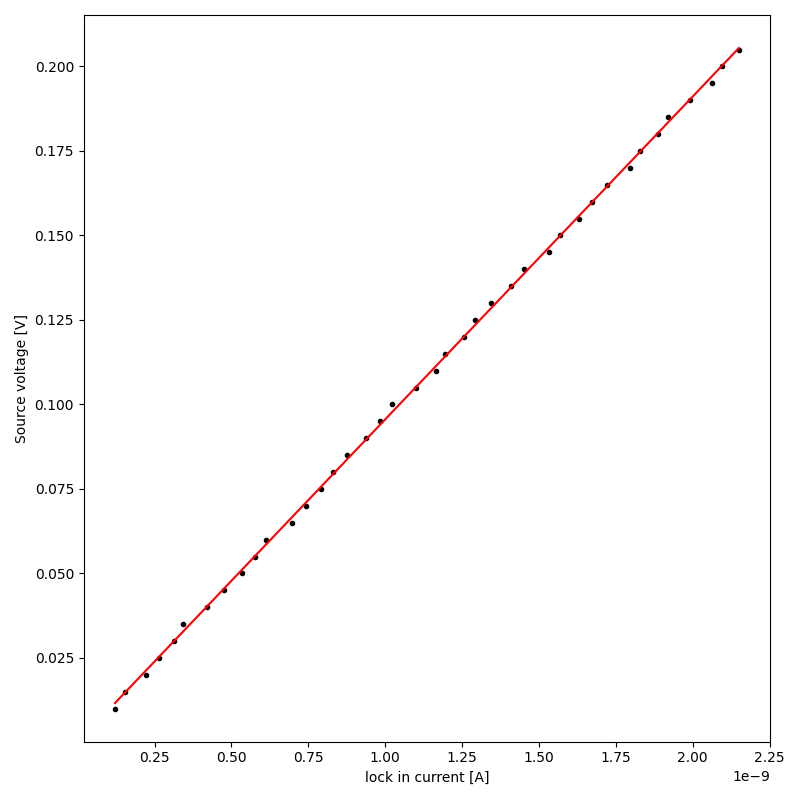
\includegraphics[width=7cm]{./figs/V-I fitted plot at 1[kHz], 100MOhm.png}
        \caption{}
    \end{subfigure}
    \begin{subfigure}[b]{7cm}
        \centering
        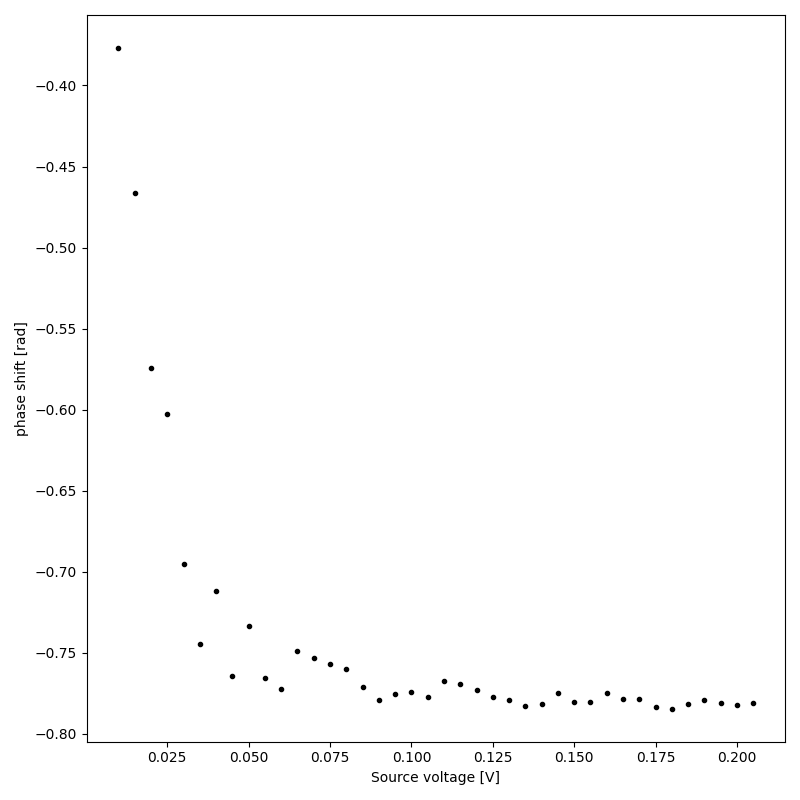
\includegraphics[width=7cm]{./figs/phi-V raw figure at 1[kHz], 100MOhm.png}
        \caption{}
    \end{subfigure}
    \hfill
    \caption{
        The lock-in detection result after the error correction by \ref{subsection: Noise Floor Detection} has been done.
        (a) is the input Voltage [V] - lock in current [A] plot. The red line is the linear regression result and the coefficient is discussed above.
        (b) measured phase shift[rad] - input Voltage [V] plot in $100M\Omega$, on the amplifier gain of $10^8 V/A$ both.
    }
    \label{fig: resistance measurement result}
\end{figure}

\section{Conclusion}
Throughout the report, the custom amplifier system is examined in two important methods.
The noise floor and its order are discussed, and the real measurement shows the experiment setup is valid enough to progress on the furthermore tests.
The noise floor of 5 [m] scale cable and 300 [K] temperature, the certain setup has 0.4 [mV] of inevitable error.
With the refined control of the error, the resistance measurement allows to calculation of the internal system resistance of an unknown custom amplifier.
The amplifier can be assumed to have a resistance in the order of $100M \Omega$, therefore the sample resistance afterward should be selected small enough to be neglected.
The lock-in detection in digital calculation is performed, so that the Visa communication is better understood.

\bibliography{noise_floor_estimation_ref}
\bibliographystyle{plain}

\end{document}